\section{Đánh giá mô hình}
\subsection{Thông số huấn luyện}
Mô hình được huấn luyện với các thông số như sau:
\begin{itemize}
    \item Tập tin pretrain: YOLOv10 - N
    \item Số batch: 32
    \item Số epoch: 50
\end{itemize}

\subsection{Kết quả huấn luyện}
\subsubsection{Thông tin chung}
\begin{itemize}
    \item \textbf{Thời gian huấn luyện:} 14.22 phút
    \item \textbf{Kích thước file pretrain sau huấn luyện:} 5.8 MB
    \item \textbf{Số lớp:} 258
    \item \textbf{Số tham số:} 2,695,586
\end{itemize}
\subsubsection{Kết quả đánh giá trên tập kiểm tra}

\begin{table}[H]
\centering
\begin{tabular}{|c|c|c|c|c|c|c|}
\hline
\textbf{Name}&\textbf{No. Img} & \textbf{No. Ins} & \textbf{Precision (P)} & \textbf{Recall (R)} & \textbf{mAP@50} & \textbf{mAP@50-95} \\ \hline
All &161 & 161 & 0.926 & 0.954 & 0.982 & 0.877 \\ \hline
Sofa & 161 & 23  & 0.882 & 0.975 & 0.977 & 0.893 \\ \hline
Table & 161 & 138 & 0.970 & 0.933 & 0.987 & 0.860 \\ \hline
\end{tabular}
\caption{Hiệu suất của mô hình trên tập kiểm tra với các lớp khác nhau}
\label{tab:performance_with_H_tag}
\end{table}

Giải thích ý nghĩa các ô trong bảng:
\begin{itemize}
    \item \textbf{Name: }Tên lớp
    \item \textbf{No. Img:} Số ảnh được kiểm tra
    \item \textbf{No. Ins: }Số đối tượng (instance) được kiểm tra
    \item \textbf{Precision (P):} khả năng phân loại đúng khi mô hình dự đoán.
    \item \textbf{Recall (R):} khả năng phát hiện các đối tượng thực tế.
    \item \textbf{mAP@50:} độ chính xác trung bình tại ngưỡng IoU 50\%.
    \item \textbf{mAP@50-95:} độ chính xác trung bình trên các ngưỡng IoU từ 50\% đến 95\%
\end{itemize}

\subsubsection{Thời gian xử lý}
Kết quả đo thời gian xử lí trung bình trên mỗi ảnh:
    \begin{itemize}
        \item \textbf{Preprocess} - tiền xử lí ảnh trước khi vào mô hình: 0.3 ms.
        \item \textbf{Inference} - thực hiện dự đoán trên dữ liệu đầu vào: 5.5 ms.
        \item \textbf{Loss} - đo lường sự khác biệt giữa dự đoán của mô hình và giá trị thực tế: 0.0 ms.
        \item \textbf{Postprocess} - xử lý và xuất ảnh đẫ dự đoán: 0.1 ms.
    \end{itemize}
Tổng thời gian xử lý: 5.9 ms/ảnh

\subsubsection{Nhận xét}

Ưu điểm:
\begin{itemize}
    \item Độ chính xác cao với mAP@50 đạt 98.2\%.
    \item Tốc độ xử lý nhanh (5.9 ms/ảnh), phù hợp với ứng dụng thời gian thực.
    \item Kích thước mô hình nhỏ gọn, dễ triển khai trên thiết bị hạn chế tài nguyên.
\end{itemize}
Hạn chế:
\begin{itemize}
    \item Thiếu tập ảnh đối tượng \textbf{chair} trong tập test, không thể đánh giá hiệu suất của lớp này.
    \item mAP@50-95 thấp hơn đáng kể (chỉ đạt 87.7\% so với 98.2\% ở mAP@50).
    \item Precision của lớp Sofa thấp hơn Recall, cần giảm số lượng dự đoán thừa (false positives).
\end{itemize}

\subsection{Kết quả dự đoán của mô hình}
Dưới đây là ảnh đã được mô hình dự đoán sau khi huấn luyện 
\begin{figure}[H]
\centering
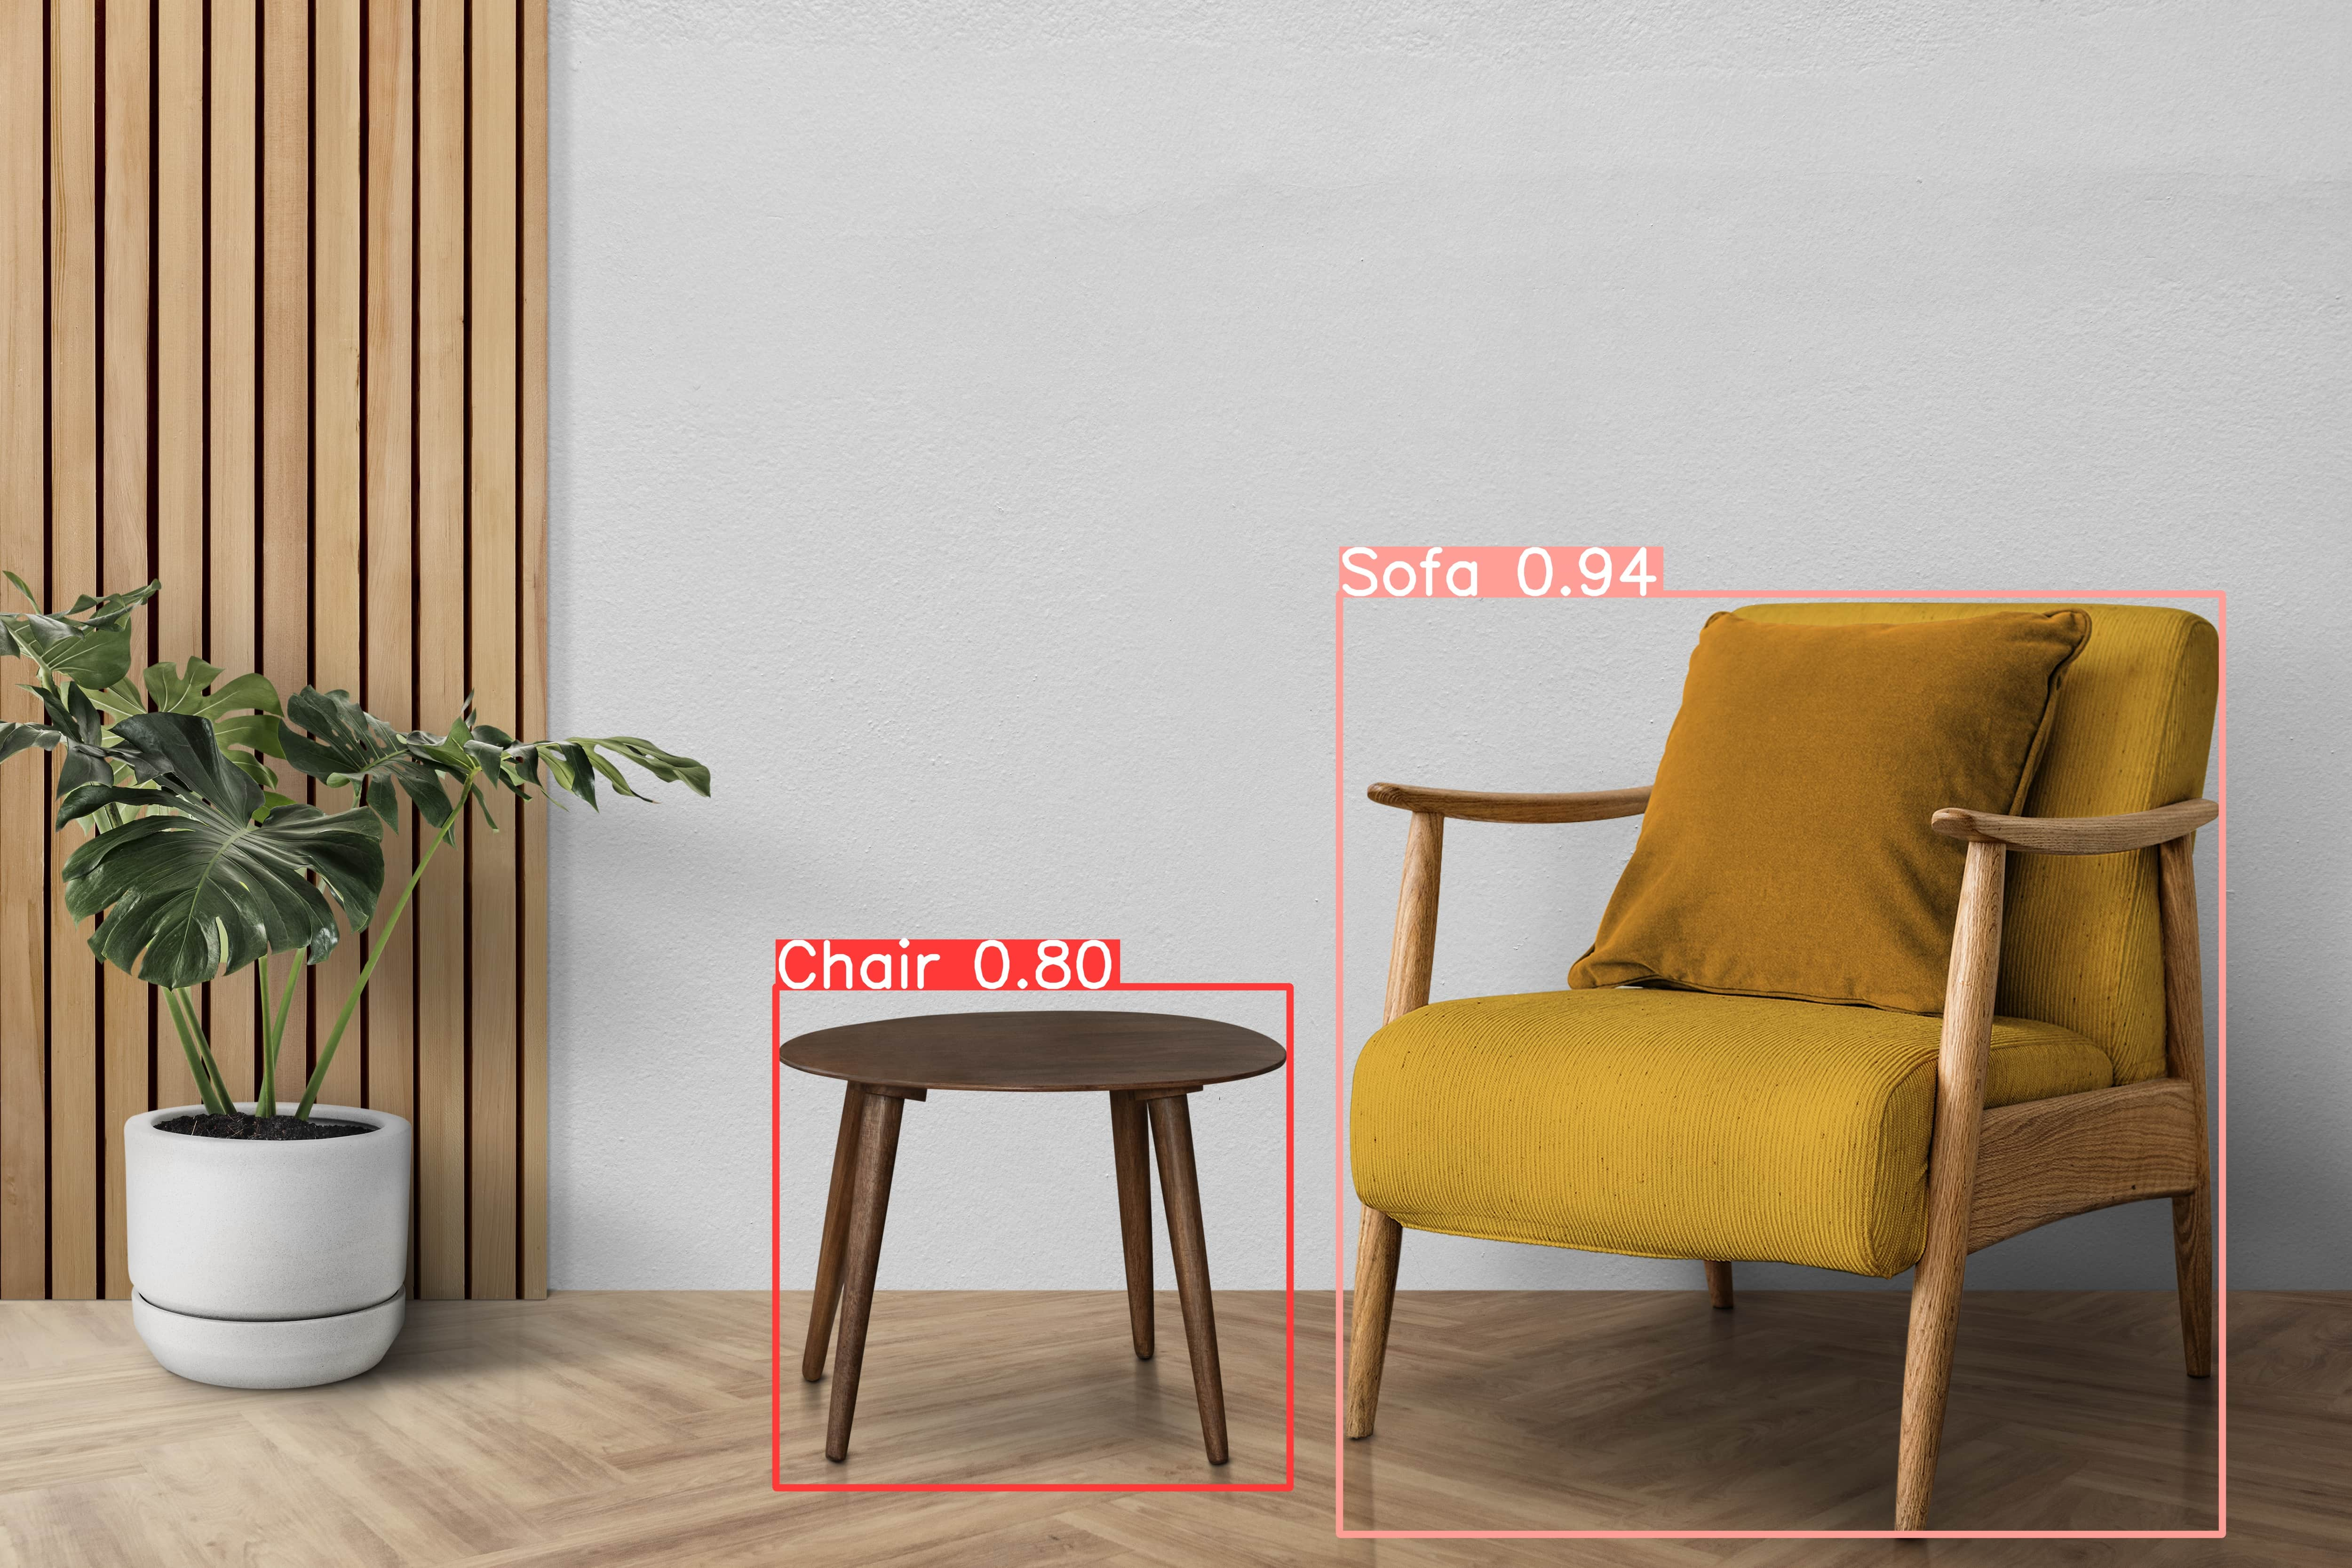
\includegraphics[scale=.08]{img/result.jpg}
\caption{Kết quả dự đoán của mô hình sau khi huấn luyện}
\label{fig:my_label_with_H}
\end{figure}



